\documentclass[../main.tex]{subfiles}


\begin{document}
\chapter{Nominal Rigidity}
    
    \section{IS-LM curve with fixed prices}
    
        Assume \textbf{firms} produce output using only labor,
        \begin{align}
            Y = F(L), \quad F'(\cdot) > 0, \quad F''(\cdot) \le 0.
        \end{align}
        All output is consumed $Y_t = C_t$ since no capital or government spending. Household gains utility from holding money, and maximizes
        \begin{align}
            \mathcal{U} &= \sum_{t=0}^\infty \beta^t
            \left[
                U(C_t) + \Gamma\left(\frac{M_t}{P_t}\right) - V(L_t)
            \right],
            \label{eqn:nom-rig-utility}
            \\
            s.t. & \quad \sum_{t=0}^\infty \frac{C_t}{\prod_{s=0}^{t}(1+r_s)}
            \le \sum_{t=0}^\infty \frac{W_t L_t}{\prod_{s=0}^{t}(1+r_s)},
            \\
            U'(\cdot),\; \Gamma'(\cdot)
            &> 0,
            \quad
            U''(\cdot),\; \Gamma''(\cdot)
            < 0,
            \quad
            V'(\cdot),\; V''(\cdot) > 0,
        \end{align}
        
        where $C_t$ is consumption, $L_t$ is labor, $W_t$ is wages, $M_t$ is money holdings, $P_t$ is fixed aggregate price, $U(\cdot), \Gamma(\cdot)$ are increasing concave functions, and $V(\cdot)$ is increasing and convex.
        
        We call $M_t / P_t$ the \textbf{real money demand}. The \textbf{real interest rate} is defined as
        \begin{align}
            1 + r_t &= \frac{1+i}{1+\pi_t},
            \quad
            1 + \pi = \frac{P_{t+1}}{P_t}
        \end{align}
        where $i_t$ is \textbf{nominal interest} and $\pi_t$ is the \textbf{inflation rate}. Household holds wealth in two assets: money $M_t$ which pays no interest, and bonds which pay $i_t$. Evolution of wealth $A$ is then
        \begin{align}
            A_{t+1} = M_t + (1+i_t)(A_t + W_t L_t - P_t C_t - M_t).
            \label{eqn:wealth-evo}
        \end{align}
        
        where $C_t$ is consumption, $L_t$ is labor, and $W_t$ is wages. Assume CRRA utility for $U(\cdot)$ and $\Gamma(\cdot)$:
        \begin{align}
            U(C_t) = \frac{C_t^{1-\theta}}{1-\theta},
            \quad
            \Gamma\left(\frac{M_t}{P_t}\right) = \frac{(M_t/P_t)^{1-\chi}}{1-\chi},
            \quad \theta,\; \chi > 0.
        \end{align}
        
    \subsection{Optimal intertemporal consumption choice}
    
        Maximizing consumption, Euler equation is
        \begin{align}
            C_t^{-\theta} = \beta (1+r_t) C_{t+1}^{-\theta}
            \label{eqn:euler-consumption}
        \end{align}
        See appendix \eqref{calc:euler-consumption} for calculation.
        Taking logs, we have that
        \begin{align}
            \ln C_t &= -\frac{\beta + \ln(1+r_{t+1})}{\theta} + \ln C_{t+1}
        \end{align}
        
        With $Y_t = C_t$ and taking $r \simeq \ln(1+r)$ as equal for small interest rates. Then
        \begin{align}
            \ln Y_t &= a + \ln Y_{t+1} - \frac{r_t}{\theta},
            \quad
            a = -\frac{\ln \beta}{\theta}
            \label{eqn:NKIS}
        \end{align}
        Equation \eqref{eqn:NKIS} is the \textbf{New Keynesian IS (Investment-Savings) Curve}, which implies an inverse relationship between output $Y_t$ and real interest rate $r_t$.\footnote{Since $\frac{\partial \ln Y_t}{\partial r_t} = \frac{1}{Y_t} \frac{\partial Y_t}{\partial r_t}
            = - \frac{1}{\theta} \implies
            \frac{\partial Y_t}{\partial r_t} = -\frac{Y_t}{\theta} < 0.$}
            
    \subsection{Optimal real money demand and consumption choice}
        From the wealth evolution \eqref{eqn:wealth-evo} and the household optimization problem \eqref{eqn:nom-rig-utility}, optimal money holdings is given by the condition
        \begin{align}
            \Gamma'\left(\frac{M_t}{P_t}\right)
            = \frac{i_t}{1+i_t}U'(C_t)
        \end{align}
        
        Then with CRRA utility for $\Gamma(\cdot)$ and $C_t = Y_t$, we have
        \begin{align}
            \frac{M_t}{P_t} = Y_t^{\theta/\chi} \left(\frac{1+i_t}{i_t}\right)^{1/\chi},
            \label{eqn:NKLM}
        \end{align}
        
        which gives us the is the \textbf{LM (liquidity-money supply) curve}. See calculations in \eqref{calc:NKLM}. Note that nominal interest rate $i_t \simeq r_t + \pi_t$ for small values. Then in the LM curve, $Y_t$ is directly proportional to $r_t$ (can show that $\frac{\partial M_t/P_t}{\partial r_t} > 0$). We also have that
        
    \subsection{Optimal labor choices}
        Optimizing between within-period consumption and labor, we have that
        \begin{align}
            C_t^{-\theta}\frac{W_t}{P_t} = V'(L_t),
            \quad V''(\cdot) > 0.
            \label{eqn:NKCL}
        \end{align}
        
        Optimal intertemporal labor choices follows:
        \begin{align}
            \frac{V'(L_t)}{V'(L_{t+1})}
            =
            \frac{W_t}{ W_{t+1}}\beta(1+r_{t+1}).
            \label{eqn:ng-labor-euler}
        \end{align}
    
    \section{Nominal rigidities}
        
        In absence of nominal rigidity or imperfections, a change in money supply leads to change in prices and wages with real wages remaining the same:
        \newcommand{\up}{\textcolor{blue}{\uparrow}}
        \newcommand{\down}{\textcolor{red}{\downarrow}}
        \begin{align}
            \frac{M \up}{P \up} = Y^{\theta/\chi} \left(\frac{1+i}{i}\right)^{1/\chi}
            \implies
            C^{-\theta}\frac{W \up}{P \up} = V'(L).
        \end{align}
        
        However, if prices are fixed $P = \bar P$ for all periods, Then by \hyperref[fig:6.2]{Figure 6.2} we have
        \begin{align}
            \frac{M \up}{\bar P} = Y^{\theta/\chi} \up \left(\frac{1+i}{i}\right)^{1/\chi}
        \end{align}
        
        \begin{figure}[ht!]
            \centering 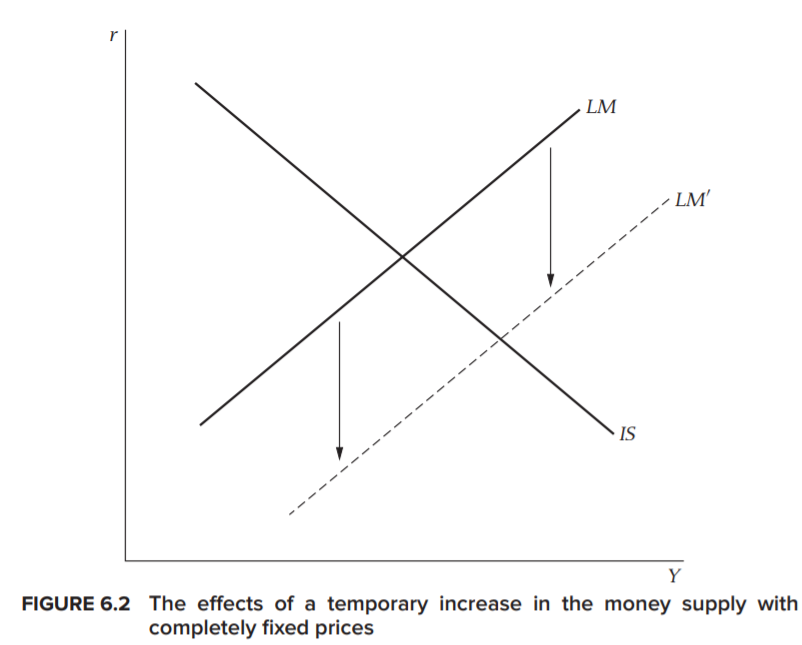
\includegraphics[width=0.65\textwidth]{./attachments/6.1-ISLM.png}
            \label{fig:6.2}
        \end{figure}
        
        This movement along the NKIS curve is a demand effect. Why do firms supply additional output? Consider four cases.
        
    \subsection*{Case 1: Keynes's General Theory}
        \emph{Goods market competitive, but rigidities in labor market.}
        
        \vspace{0.25cm}
        
        Assume flexible prices and wages are fixed above natural level. Output is a function of labor, and firms maximize $F(L) - \frac{W}{P}L$.
        \begin{align}
            W = \bar W,
            \quad
            Y = F(L) \implies F'(L)
            = \frac{\bar W}{P},
            \quad
            F''(\cdot) \leq 0.
        \end{align}
        
        With wages above natural level, we have equilibrium at point E in \hyperref[fig:6.3]{Figure 6.3}.
        
        \begin{figure}[h!]
            \centering
            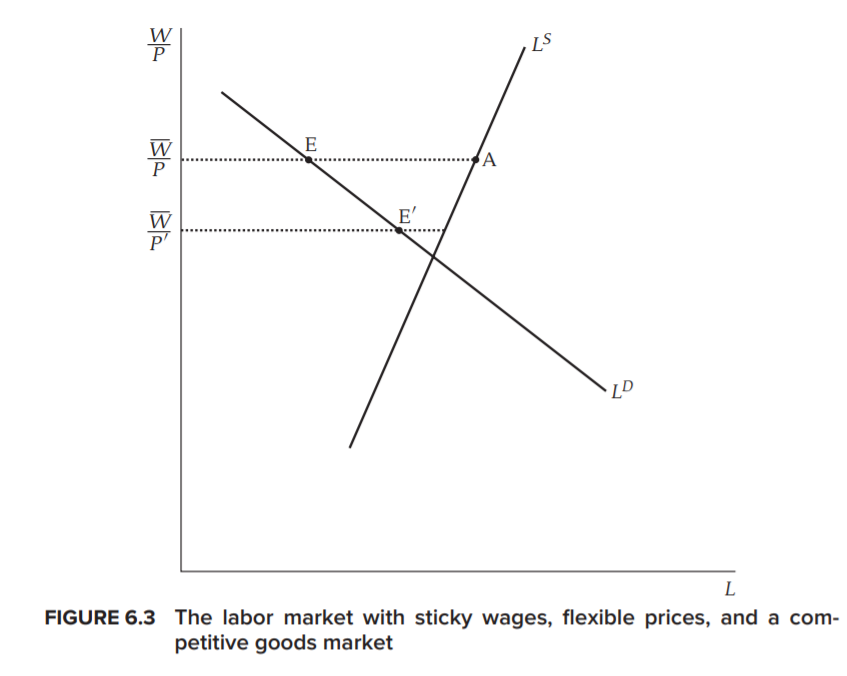
\includegraphics[width=0.65\textwidth]{./attachments/6.2-case1.png}
            \label{fig:6.3}
        \end{figure}
        
        Then with a money supply increase, good prices increase, real wages fall, and employment rises to E' in \hyperref[fig:6.3]{Figure 6.3}:
        \begin{align}
            \frac{M \up}{P \up} = Y^{\theta/\chi} \left(\frac{1+i}{i}\right)^{1/\chi}
            \implies
            \frac{\bar W}{P \up}
            = F'(L) \down,
            \; F''(L) \le 0
            &\implies
            F'(L \up)
            \\
            &\implies
            Y \up = F(L \up).
        \end{align}
        
    \subsection*{Case 2: Sticky prices, flexible wages, competitive labor market}
        \emph{Labor market competitive, but rigidities in goods market.}
    
        \vspace{0.25cm}
        
        Assume prices fixed, wages flexible. Workers maximize within-period consumption labor trade off as in \eqref{eqn:NKCL}. In market equilibrium, $C = Y = F(L)$. Then we have
        \begin{align}
            \frac{W}{\bar P}
            = F(L)^{\theta} V'(L).
        \end{align}
        
        Then if money supply increases with fixed prices, goods demand increases, labor demand increases to meet the goods demand, and wages rise, illustrated in Figure 6.4:
        \begin{align}
            \frac{M \up}{\bar P} = Y^{\theta/\chi} \up \left(\frac{1+i}{i}\right)^{1/\chi}
            \implies
            Y \up = F(L \up), \; F'(\cdot) > 0
            \implies
            F(L)^{\theta} \up V'(L)
            =\frac{W \up}{\bar P}.
        \end{align}
        
        \begin{figure}[h!]
            \centering
            \begin{subfigure}   
                \centering
                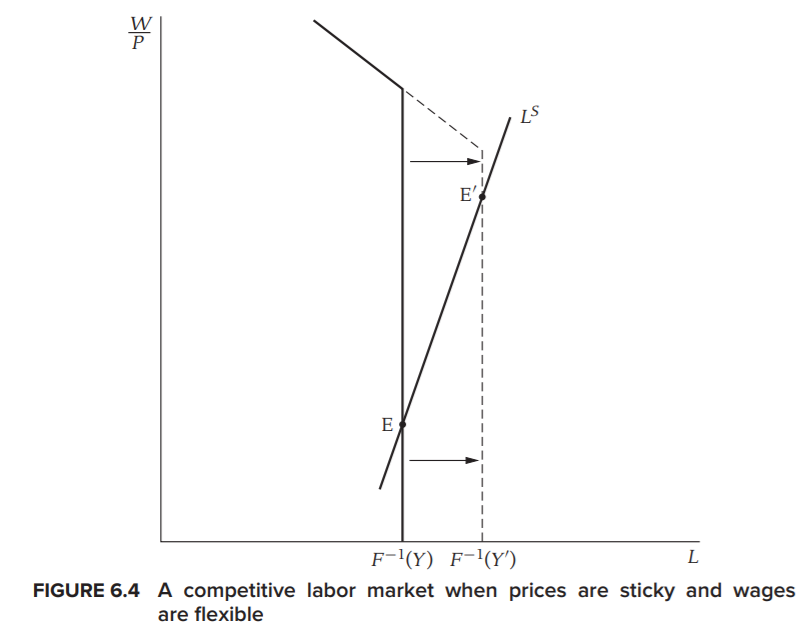
\includegraphics[width=0.45\textwidth]{./attachments/6.3-case2.png}
            \end{subfigure}
            \begin{subfigure}  
                \centering
                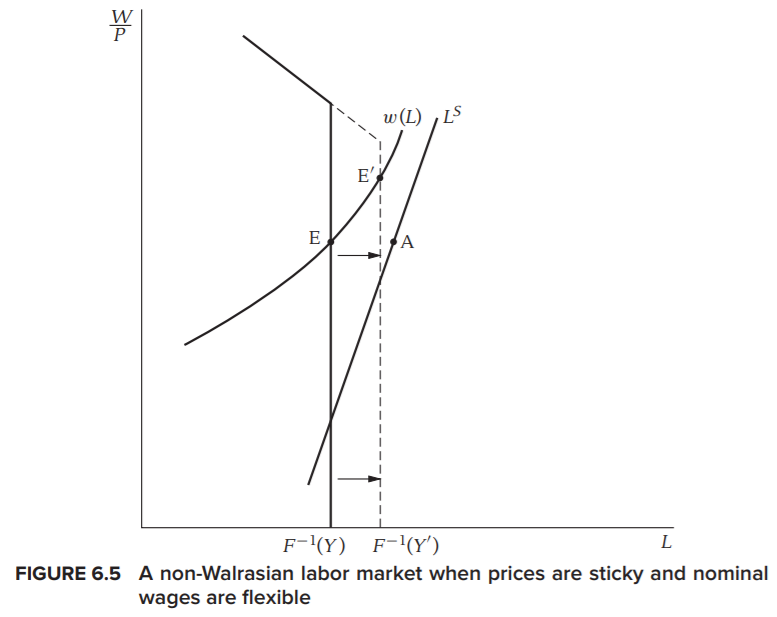
\includegraphics[width=0.45\textwidth]{./attachments/6.4-case3.png}
            \end{subfigure}
            \label{fig:6.4}
        \end{figure}
        
    \subsection*{Case 3: Sticky prices, flexible wages, real labor market imperfections}
        
        Same setup and mechanisms as Case 2, but with non-Walrasian labor market where real wage remains above level that equates supply and demand (Figure 6.5).
        
    \subsection*{Case 4: Sticky wages, flexible prices, imperfect competition}
    
        Assume wages are rigid $W = \bar W$. Prices are flexible but imperfectly competitive, given by
        \begin{align}
            P = \mu(L) \frac{\bar W}{F'(L)}
            \implies
            \frac{\bar W}{P} = \frac{F'(L)}{\mu(L)}
        \end{align}
        
        where $\mu(L)$ is a markup function. Since $F''(L) \le 0$, labor demand then depends on $\mu'(\cdot)$, whether markup increases or decreases with labor demand:
        \begin{align}
            \frac{M \up}{P \up} = Y^{\theta/\chi} \left(\frac{1+i}{i}\right)^{1/\chi}
            \implies
            \frac{\bar W}{P \up}
            = \frac{F'(L)}{\mu(L)} \down
            \implies
            F(L) = Y \up \down ?
        \end{align}
        The markup function $\mu(L)$ is a feature of imperfect competition, which we examine next.
        
    %% section on output-inflation trade-off, natural rate hypothesis, accelerationist Phillips curve. Romer pg 256 (pdf 275)
    
    \section{Imperfect competition}
        
        Assume a continuum of firms $i \in [0, 1]$ producing unique goods with production functions
        \begin{align}
            Y_{i} = L_{i}
            \label{eqn:imperfect-prod-fn}
        \end{align}
        Representative household maximizes utility
        \begin{align}
            U &= C - \frac{1}{\gamma} L^{\gamma}, \quad \gamma > 1,
            \\
            C &= \left[
                \int_{i=0}^1 C_i^{(\eta - 1)/\eta} di
            \right]^{\eta / (\eta - 1)},
            \quad \eta > 1.
            \label{eqn:impcomp-consumption-utility}
        \end{align}
        where $C$ is the CES consumption index. With no investment or government spending, we use $Y = C$ as measure of output in the economy. Assumption for simplicity output is equal to money demand:
        \begin{align}
            Y = \frac{M}{P}.
        \end{align}
        
    \subsection{Households}
        
        Let $S$ be the household's total spending budget. Household's Lagrangian is then
        \begin{align}
            \L = \left(
                    \int_{i=0}^1 C_i^{(\eta - 1)/\eta} di
                \right)^{\eta / (\eta - 1)}
            - \frac{1}{\gamma} L^{\gamma}
            +\lambda \left(
                S - \int_{i=0}^1 P_i C_i di
            \right).
        \end{align}
        
        Optimizing consumption, we have the FOC
        \begin{align}
            \frac{\partial \L}{\partial C_i} = 0
            &\implies 
            \frac{\eta}{\eta - 1} \left(
                    \int_{j=0}^1 C_j^{(\eta - 1)/\eta} dj
                \right)^{1 / (\eta - 1)} C_i^{\frac{- 1}{\eta}} \frac{\eta - 1}{\eta}
            = \lambda P_i
            \\
            &\implies
            \left(
                    \int_{j=0}^1 C_j^{(\eta - 1)/\eta} dj
                \right)^{1 / (\eta - 1)} C_i^{\frac{- 1}{\eta}}
            = \lambda P_i
            \\
            &\implies
            C_i = A P_i^{-\eta}
            \label{eqn:impcom-consumption}
        \end{align}
        for some $A$ which is constant across firms $i$. Plugging \eqref{eqn:impcom-consumption} into the budget constraint,
        we have
        \begin{align}
            S
            = \int_{j=0}^1 P_j C_j dj
            = \int_{j=0}^1 P_j (A  P_j^{-\eta}) dj
            &= A \int_{j=0}^1 P_j^{1-\eta} dj
            \\ \implies
            A
            &= \frac{S}{\int_{j=0}^1 P_j^{(1-\eta)} dj}.
            \label{eqn:A}
        \end{align}
        
        Then we have that
        \begin{align}
            C
            = \left[
                    \int_{i=0}^1 C_i^{(\eta - 1)/\eta} di
                \right]^{\eta / (\eta - 1)}
            = \frac{S}{P},
            \quad
            P = \left[
                \int_{i=0}^1
                P_i^{(1-\eta)}
                di
                \right]^{\frac{1}{1 - \eta}},
            \label{eqn:price-index}
        \end{align}
        where $P$ is the price index corresponding to consumption utility. See appendix \eqref{calc:price-index} for full derivations. Then we have by \eqref{eqn:impcom-consumption}, \eqref{eqn:A}, and \eqref{eqn:price-index} that
        \begin{align}
            C_i = A P_i^{-\eta}
            = \frac{S}{P^{1-\eta}} P_i^{-\eta}
            = \frac{S}{P} \left(\frac{P_i}{P}\right)^{-\eta}
            = C \left(\frac{P_i}{P}\right)^{-\eta}.
            \label{eqn:consumption-demand}
        \end{align}
        
    \subsection{Firms}
    
        Our production function is $Y_i = L_i$. Firm $i$ maximizes real profits by choosing prices:
        \begin{align}
            \max_{P_i} R_i &= \frac{P_i Y_i}{P} - \frac{W L_i}{P}
            = \frac{P_i Y_i}{P} - \frac{W Y_i}{P}
            \\
            &= \frac{P_i Y \left(\frac{P_i}{P}\right)^{-\eta}}{P} - \frac{W Y \left(\frac{P_i}{P}\right)^{-\eta}}{P}
            \\
            &= Y \left(\frac{{P_i}}{P}\right)^{1-\eta} - \frac{WY}{P} \left(\frac{{P_i}}{P}\right)^{-\eta}
        \end{align}
        
        FOC with respect to $\frac{P_i}{P}$:
        \begin{align}
            \frac{\partial R_i}{\partial (P_i / P)} = 0
            &\implies 
            (\eta-1) Y \left(\frac{{P_i}}{P}\right)^{-\eta} 
            = \eta \frac{WY}{P} \left(\frac{{P_i}}{P}\right)^{-\eta-1}
            \\
            &\implies
            \frac{P_i}{P} = \frac{W}{P} \frac{\eta}{\eta-1}.
            \label{eqn:markup-price}
        \end{align}
        
        In perfect competition the firm would be a price taker maximizing profit by choosing $Y_i$, which implies $\frac{P_i}{P} = \frac{W}{P}$, the marginal cost. With imperfect competition, $\frac{\eta}{\eta - 1}$ becomes the markup factor over the perfect competition price. Notice that if $\eta \to -\infty$ then $\frac{P_i}{P} \to \frac{W}{P}$.
        
    
    % appendix
    \renewcommand{\thesection}{A\arabic{chapter}}
    
    \newpage
    \section{Appendix}
    
    \subsection{CRRA euler utility derivation eq (\ref{eqn:euler-consumption})}\label{calc:euler-consumption}
        
        \begin{align}
            \L(C_t, M_t, \lambda)
            &= \sum_{t=0}^\infty \beta^t
            \left[
                \frac{C_t^{1-\theta}}{1-\theta}
                + \frac{(M_t/P_t)^{1-\chi}}{1-\chi}
                - V(L_t)
            \right] \\
            &\quad + \lambda \left(
                \sum_{t=0}^\infty \frac{W_t L_t}{\prod_{s=0}^{t}(1+r_s)} - \frac{C_t}{\prod_{s=0}^{t}(1+r_s)}
            \right).
            \\
            \frac{\partial\L}{\partial C_t} = 0
            &\implies \beta^t C_t^{-\theta}
            = \frac{\lambda}{\prod_{s=0}^{t}(1+r_s)}
            \\
            &\implies
            \frac{\beta^t C_t^{-\theta}}{\beta^{t+1} C_{t+1}^{-\theta}}
            =  \frac{\lambda \prod_{s=0}^{t+1}(1+r_s)}{\lambda \prod_{s=0}^{t}(1+r_s)}
            \\
            &\implies
            C_t^{-\theta}
            =  \beta (1+r_{t+1}) C_{t+1}^{-\theta}
        \end{align}
        
        Change time indexing convention for $r_{t+1}$ to one period prior. $r_{t}$ is the interest to be paid out at $t+1$. Then the Euler equation is
        \begin{align}
            C_t^{-\theta}
            =  \beta (1+r_t) C_{t+1}^{-\theta}.
        \end{align}
    
    
    \subsection{LM Curve derivation eq (\ref{eqn:NKLM})}\label{calc:NKLM}
        
        Holding wealth $A_{t+1}$ constant, from \eqref{eqn:wealth-evo} we have the following from a small change $\Delta M$ in period $t$ money supply:
        \begin{align}
            A_{t+1}
            &= M_t + (1+i_t)(A_t + W_t L_t - P_t C_t - M_t)
            \\
            &= [M_t + \Delta m]
            + (1+i_t)\left(
              A_t + W_t L_t
              - P_t \left[C_t - \frac{i_t}{(1+i_t)}\frac{1}{P_t} \Delta m\right]
              - [M_t + \Delta m]
              \right)
        \end{align}
        
        Thus a change of $dM = \Delta m$ in $M_t$ results in a change of $dC = -\frac{i_t}{(1+i_t)}\frac{1}{P_t} \Delta m$ in $C_t$ within the same budget.
        Then on the optimal path, with $C_t = Y_t$
        \begin{align}
            d \mathcal{U} = 0
            &= \Gamma'(M_t / P_t)\frac{1}{P_t} dM + U'(C_t)dC
            \\
            &= (M_t / P_t)^{-\chi} \frac{1}{P_t} dM + C_t^{-\theta} dC
            \\
            &= (M_t / P_t)^{-\chi} \frac{1}{P_t} \Delta m
            -C_t^{-\theta}
            \frac{i_t}{(1+i_t) }\frac{1}{P_t} \Delta m
            \\
            \implies
            (M_t / P_t)^{-\chi}
            &= Y_t^{-\theta} \frac{i_t}{1+i_t}
            \\
            \implies
            \frac{M_t}{P_t}
            &= Y_t^{\theta/\chi} \left(\frac{1+i_t}{i_t}\right)^{1/\chi}.
        \end{align}
    
    \subsection{Optimal price index derivation eq  (\ref{eqn:price-index})}\label{calc:price-index}
    
        From \eqref{eqn:impcom-consumption} we have $C_i = A P_i^{-\eta}$, and from \eqref{eqn:A} we have $A = \frac{S}{\int_{j=0}^1 P_j^{(1-\eta)} dj}$. Then with the definition of aggregate consumption $C$ from \eqref{eqn:impcomp-consumption-utility}, we have
        \begin{align}
            C = \left[
                    \int_{i=0}^1 C_i^{(\eta - 1)/\eta} di
                \right]^{\eta / (\eta - 1)}
            &= \left[
                \int_{i=0}^1 (A P_i^{-\eta})^{(\eta - 1)/\eta} di
                \right]^{\eta / (\eta - 1)}
            \\
            &= \left[
                \int_{i=0}^1 A^{(\eta - 1)/\eta} P_i^{(1-\eta)} di
                \right]^{\eta / (\eta - 1)}
            \\
            &= \left[
                \int_{i=0}^1
                \left(\frac{S}{\int_{j=0}^1 P_j^{(1-\eta)} dj}\right)^{(\eta - 1)/\eta}
                P_i^{(1-\eta)}
                di
                \right]^{\eta / (\eta - 1)}
            \\
            &= \frac{S}{\int_{j=0}^1 P_j^{(1-\eta)} dj}
                \left[
                \int_{i=0}^1
                P_i^{(1-\eta)}
                di
                \right]^{\eta / (\eta - 1)}
            \\
            &= \frac{S}{
                \left[
                \int_{i=0}^1
                P_i^{(1-\eta)}
                di
                \right]^{\frac{1}{1 - \eta}}
                }
            = \frac{S}{P},
            \quad P \equiv \left[
                \int_{i=0}^1
                P_i^{(1-\eta)}
                di
                \right]^{\frac{1}{1 - \eta}}.
        \end{align}
        
        
    % reset sections
    \renewcommand{\thesection}{\arabic{chapter}.\arabic{section}}
    
    \chapter{Dynamic Stochastic General Equilibrium Models (DSGE)}
        
    \section{Households}
        Representative household maximizes utility
        \begin{align}
            \mathcal{U} &= \sum_{t=0}^{\infty} \beta^{t} [U(C_t) - V(L_t)]
            \quad \beta \in (0, 1),
            \\
            s.t. \quad &
            \sum_{t=0}^{\infty} \frac{P_t C_t}{\prod_{s=0}^{t}(1+r_{s})} \le
            \sum_{t=0}^{\infty} \frac{W_t L_t}{\prod_{s=0}^{t}(1+r_{s})}
        \end{align}
        
        where
        \begin{align}
            U(C_t) &= \frac{C_t^{1-\theta}}{1-\theta},
            \quad
            V(L_t) = \frac{B}{\gamma} L_t^\gamma, 
            \quad 
            \theta, B, \gamma > 0
            \\
            \implies
            U'(C_t) &= C_t^{-\theta},
            \quad
            V'(L_t) = B L_t^{\gamma - 1}.
        \end{align}
        
        Forming Lagrangian, we have
        \begin{align}
            \L &= \sum_{t=0}^{\infty} \beta^{t} [U(C_t) - V(L_t)] + \lambda 
            \left(
                \sum_{t=0}^{\infty} \frac{W_t L_t}{\prod_{s=0}^{t}(1+r_{s})}
                - 
                \sum_{t=0}^{\infty} \frac{C_t}{\prod_{s=0}^{t}(1+r_{s})}
            \right).
        \end{align}
        
        We have the following from the FOCs:
        \begin{align}
            \frac{\partial \L}{\partial L_t} = 0
            &\implies
            \beta^t V'(L_t) = \frac{\lambda W_t}{\prod_{s=0}^{t}(1+r_{s})},
            \\
            \frac{\partial \L}{\partial C_t} = 0
            &\implies
            \beta^t U'(C_t) = \frac{\lambda P_t}{\prod_{s=0}^{t}(1+r_{s})},
            \\
            &\implies
            \frac{W_t}{P_t} = \frac{V'(L_t)}{U'(C_t)}
            = \frac{BL_t^{\gamma - 1}}{C_t^{-\theta}}
            % = BL_t^{\gamma - 1}C_t^{\theta}
            = B Y_t ^{\theta + \gamma - 1}
            \label{eqn:dsge-eqm-wage}
        \end{align}
        
        since we assume that $Y_t = F(L_t) = L_t = C_t$. % Our assumptions about consumption are same as in \eqref{eqn:NKIS}, thus again we have
        % \begin{align}
        %     \ln Y_t &= a + \ln Y_{t+1} - \frac{r_t}{\theta}.
        % \end{align}
        
    
    \section{Firms}
    
        Firm producing good $i$ has production function
        \begin{align}
            Y_{it} = L_{it}
        \end{align}
        and by \eqref{eqn:consumption-demand} is met with demand
        \begin{align}
            Y_{it} = Y_t \left(\frac{P_{it}}{Pt}\right)^{-\eta}.
            \label{eqn:markup-demand}
        \end{align}
        
        Firm $i$ sets price $p_i$ in period 0. The firm's real profit in period $t$ is
        \begin{align}
            R_{it}(P_i)
            &= \frac{P_i}{P}Y_{it} - \frac{W}{P} L_{it}
            = \frac{P_i}{P}Y_{it} - \frac{W}{P} Y_{it}
            \\
            &=
            Y_t \left(\frac{{P_i}}{P_t}\right)^{1-\eta} - \frac{W_tY_t}{P_t} \left(\frac{{P_i}}{P_t}\right)^{-\eta}
        \end{align}
        
    \section{Sticky Prices}
    
        Let $q_t$ be the probability that the price the firm sets in period $0$ stays the same in period $t$. Define the stochastic discount factor (SDF):
        \begin{align}
            \lambda_t = \beta^t \frac{U'(C_t)}{U'(C_0)}.
        \end{align}
        % (?) which comes from Lagrangian
        % \begin{align}
        %     \max_{\{C_t\}_{t=0}^\infty, \{L_t\}_{t=0}^\infty} &
        %     \sum_{t=0}^{\infty} \beta^t \left[ U(C_t) - V(L_t) \right]
        %     \quad s.t. \quad
        %     Y_t \ge C_t, \quad \forall t \in \{0, 1, 2, ...\}
        %     \\
        %     \L
        %     &= \sum_{t=0}^{\infty} \beta^t \left[ U(C_t) - V(L_t) \right] - \sum_{t=0}^\infty \lambda_t (Y_t - C_t)
        %     \\
        %     \frac{\partial \L}{\partial C_t} &= 0
        %     \implies \beta^t U'(C_t) = \lambda_t
        %     \implies \beta^t \frac{U'(C_t)}{U'(C_0)} = \frac{\lambda_t}{\lambda_0}
        % \end{align}
        
        Firm's problem is to choose $p_i$ at time $t=0$ to maximize $A$:
        \begin{align}
            \max_{P_i} A = \E{\sum_{t=0}^\infty q_t \lambda_t R_{it}}
            &= \E{\sum_{t=0}^\infty q_t \lambda_t
            \left(
                Y_t \left(\frac{{P_i}}{P_t}\right)^{1-\eta} - Y_t\frac{W_t}{P_t} \left(\frac{{P_i}}{P_t}\right)^{-\eta}
                \right)}
            \\
            &= \E{\sum_{t=0}^\infty q_t \lambda_t
            Y_t P_t^{\eta - 1}\left(
                P_i^{1-\eta} - \frac{W_t}{P_t} P_i^{-\eta}
                \right)}
            \\
            &= \E{\sum_{t=0}^\infty q_t \lambda_t
            Y_t P_t^{\eta - 1} F(p_i, p_t^*)}
        \end{align}
        where $P_t^*$ is the price that optimizes profits in period $t$.  For example, by \eqref{eqn:markup-price} $P_{it}^* = P_{t}^* = W_t\frac{\eta}{\eta-1}$ for all $i$. $F(p_t, p_t^*)$ is a function of log prices $p_i = \ln{P_i}$ and $p_t^* = \ln{P_t^*}$, where $p_i = p_t^*$ maximizes period-$t$ profits. This implies
        \begin{align}
            \frac{\partial F(p_t^*, p_t^*)}{\partial p_i} = 0,
            \quad
            \frac{\partial^2 F(p_t^*, p_t^*)}{\partial p_i^2} < 0,
        \end{align}
        
        by existence of maximum, assuming $F(p_i, p_t^*)$ is differentiable everywhere. Assume $F(p_i, p_i^*)$ can be approximated around $p_i = p_i^*$ by the second order Taylor approximation:
        \begin{align}
            F(p_i, p_i^*)
            &\simeq F(p_t^*, p_t^*) +  \frac{\partial F(p_t^*, p_t^*)}{\partial p_i} (p_i - p_t^*) + \frac{\partial^2 F(p_t^*, p_t^*)}{\partial p_i^2} (p_i - p_t^*)^2
            \\
            &= F(p_t^*, p_t^*) - K (p_i - p_t^*)^2, \quad K > 0
            \\
            \implies
            F(p_t^*, p_t^*) - F(p_i, p_i^*) &= K(p_i - p_t^*)^2.
        \end{align}
        
        Assuming fluctuations in $Y_t P_t^{\eta - 1}$ is negligible across periods compared to $q_t$ and $F(p_i, p_t^*)$, we can find the optimal $p_i = \ln P_i$ by minimzing the ``distance" between $F(p_i, p_t^*)$ and $F(p_t^*, p_t^*)$:
        \begin{align}
            p_i^*
            &= \arg\min_{p_i} \sum_{t=0}^\infty q_t \beta^t \E{F(p_i, p_t^*) - F(p^*, p^*)}
            \\
            % &= \arg\min_{p_i} \sum_{t=0}^\infty q_t \beta^t \E{(p_i - p_t^*)^2}
            % \\
            \implies p_i^*
            &= \sum_{t=0}^\infty \tilde\omega_t \E{p_t^*}, \quad
            \tilde\omega_t = \frac{\beta^t q_t}{\sum_{s=0}^\infty \beta^s q_s}
            \label{eqn:p-star}
        \end{align}
        
        See appendix \eqref{calc:p-star} for calculations. Then combining equilibrium log-wage $w_t$ from \eqref{eqn:dsge-eqm-wage} and each firm's profit-maximizing log-price in each period $p_t^*$ from \eqref{eqn:markup-price}, we have
        \begin{align}
            w_t &= p_t + \ln{B} + (\theta + \gamma - 1) y_t,
            \\
            p_t^* &= \ln{\frac{\eta}{\eta - 1}} + w_t
            \\
            &= \phi m_t + (1-\phi) p_t + c \label{eqn:optimal-price-t}
        \end{align}
        
        where $m_t = y_t + p_t$ is log-nominal GDP and
        \begin{align}
            \phi &= \theta + \gamma - 1 > 0, \quad
            c = \ln{\frac{\eta}{\eta - 1}} + \ln{B} = 0
        \end{align}
        
        See appendix \eqref{calc:optimal-price-t} for full derivation. Then firm $i$'s optimal price at time $t$ is
        \begin{align}
            p_{it}^*
            = \sum_{s=0}^\infty \tilde\omega_{t+s} \E{p_{t+s}^*}
            &= \sum_{s=0}^\infty \tilde\omega_{t+s} \E{\phi m_{t+s} + (1-\phi) p_{t+s}}.
        \end{align}
        
    \section{Calvo Model and New Keynesian Phillips Curve}
    
        Assume in every period, a random fraction $\alpha \in (0, 1]$ of firms can change prices.\footnote{Probability that price stays the same after $j$ periods are then $q_j = (1-\alpha)^j$.}
        Average prices $p_t$ and inflation $\pi_t$ in period $t$ is then
        \begin{align}
            p_t &= \alpha x_t + (1 - \alpha) p_{t-1}
            \\
            \implies
            p_t - p_{t-1}
            &= \pi_t = \alpha (x_t - p_{t-1})
            \implies
            \frac{\pi_t}{\alpha}
            = x_t - p_{t-1}
        \end{align}
        where $p_{t-1}$ is average old price and $z_t$ is new profit-mazimizing prices\footnote{$y = 1 + z + z^2 + z^3 + ... = 1 + z(1 + z + z^2 + z^3 + ...) = 1 + zy \implies y = \frac{1}{1-z}$. Then letting $z = \beta(1-\alpha)$, we have $\left(\sum_{k=0}^\infty\beta^k(1-\alpha)^k\right)^{-1} = 1-\beta(1-\alpha)$.}
        
        \begin{align}
            x_t
            &= \sum_{j=0}^\infty \tilde\omega_{j} \E{p_{t+j}^*}
            ,\quad
            \tilde\omega_j
            = \frac{\beta^j (1-\alpha)^j}{\sum_{k=0}^\infty \beta^k (1-\alpha)^k}
            = [1 - \beta(1-\alpha)] \beta^j (1-\alpha)^j q_j
            \\
            x_t
            &= [1 - \beta(1-\alpha)] \sum_{j=0}^\infty \beta^j (1-\alpha)^j \E{p_{t+j}^*}
            \\
            &= [1 - \beta(1-\alpha)] \E{p_{t}^*}
            + \beta (1-\alpha) [1 - \beta(1-\alpha)] \sum_{j=0}^\infty \beta^j (1-\alpha)^j \E{p_{(t+1)+j}^*}
            \\
            &= [1 - \beta(1-\alpha)] p_{t}^*
            + \beta (1-\alpha) \E{x_{t+1}}
        \end{align}
        
        With \eqref{eqn:optimal-price-t} we have that $p_t^* - p_t = \theta y_t$, then
        \begin{align}
            x_t - p_t
            &= [1 - \beta(1-\alpha)] (p_{t}^* - p_t)
            + \beta (1-\alpha) \E{x_{t+1} - p_t}
            \\
            &= [1 - \beta(1-\alpha)] (\phi y_t) 
            + \beta (1-\alpha) \E{\frac{\pi_{t+1}}{\alpha}}
        \end{align}
        
        We also have that
        \begin{align}
            x_t - p_t
            &= (x_t - p_{t-1}) - (p_t - p_{t-1})
            = \frac{\pi_t}{\alpha} - \pi_t
            = \pi_t \frac{1 - \alpha}{\alpha}
        \end{align}
        
        Then combining the two
        \begin{align}
            \implies
            \pi_t
            &=
            \frac{\alpha}{1-\alpha}
            [1 - \beta(1-\alpha)] \phi y_t
            + \beta \E{\pi_{t+1}}
            \\
            &= \kappa y_t + \beta \Et{\pi_{t+1}},
            \quad
            \kappa = \frac{\alpha}{1-\alpha}
            [1 - \beta(1-\alpha)] \phi, \label{eqn:nk-phillips-curve}
        \end{align}
        which is the \textbf{New Keynsian Phillips Curve}, which relates inflation to output and expected inflation.
        
        
    % appendix
    \renewcommand{\thesection}{A\arabic{chapter}}
        
    \newpage
    \section{Appendix}
        
    \subsection{Price difference minimization eq (\ref{eqn:p-star})}\label{calc:p-star}
        Expectation of the square of a random $x$ is as follows
        \begin{align}
            \E{x^2}
            &= \E{([x - \mu_x] + \mu_x)^2}
            \\
            &= \E{\mu_x^2 + (x - \mu_x)^2 + 2\mu_x(x - \mu_x)}
            \\
            &= \mu_x^2 + \E{(x - \mu_x)^2} + 2\mu_x\E{x - \mu_x}
            \\
            &= \E{x}^2 + \var{x}.
        \end{align}
    
        Then,
        \begin{align}
            p_i^*
            = \arg\min_{p_i} \sum_{t=0}^\infty q_t \beta^t \E{F(p_i, p_t^*) - F(p^*, p^*)}
            &=\sum_{t=0}^\infty q_t \beta^t \E{(p_i - p_t^*)^2}
            \\
            &= \sum_{t=0}^\infty q_t \beta^t \left[(p_i - \E{p_t^*})^2 + \var{p_t^*}\right].
        \end{align}
        
        Then finding optimal $p_i$ with the FOC:
        \begin{align}
            \frac{\partial D}{\partial p_i}
            = \sum_{t=0}^\infty 2 \beta^t q_t (p_i - \E{p_t^*})
            = 0
            &\implies
            2p_i \sum_{s=0}^\infty \beta^s q_s = 2\sum_{t=0}^\infty q_t \beta^t \E{p_t^*}
            \\
            &\implies
            p_i = \frac{\sum_{t=0}^\infty q_t \beta^t \E{p_t^*}}{\sum_{s=0}^\infty \beta^s q_s}
            = \sum_{t=0}^\infty \frac{\beta^t q_t}{\sum_{s=0}^\infty \beta^s q_s} \E{p_t^*}
            \\
            &\implies
            p_i^* = \sum_{t=0}^\infty \tilde\omega_t \E{p_t^*}, \quad \tilde\omega_t = \frac{\beta^t q_t}{\sum_{s=0}^\infty \beta^s q_s}
        \end{align}
        
    \subsection{Revenue maximizing price derivation eq (\ref{eqn:optimal-price-t})}
        \label{calc:optimal-price-t}
        
        From \eqref{eqn:dsge-eqm-wage} we have
        \begin{align}
            w_t &= p_t + \ln{B} + (\theta + \gamma - 1) y_t,
        \end{align}
        
        and from \eqref{eqn:markup-price} we have each firm's profit-maximizing log-price in each period,
        \begin{align}
            \max_{p_{it}}\ln[R_{it}(P_{it})]
            = p_t^* &= \ln{\frac{\eta}{\eta - 1}} + w_t
            \\
            &= \ln{\frac{\eta}{\eta - 1}}
            + p_t + \ln{B} + (\theta + \gamma - 1) y_t
            \\
            &= p_t + c + \phi y_t
            \\
            &= p_t + c + \phi y_t + \phi p_t - \phi p_t
            \\
            &= \phi (y_t + p_t) + (1-\phi) p_t + c
            \\
            &= \phi m_t + (1-\phi) p_t, \quad m_t = y_t + p_t, \quad c = 0
        \end{align}
        where $\phi = \theta + \gamma - 1$ and $c = \ln{\frac{\eta}{\eta - 1}} + \ln{B}$. $m_t$ is log nominal GDP $y_t + p_t$.
        
    % reset sections
    \setcounter{section}{1}
    \renewcommand{\thesection}{\arabic{chapter}.\arabic{section}}
    
    \chapter{Monetary Policy}
    
        \section{Inflation, money growth, interest rates}
        
        Model for LM curve in \eqref{eqn:NKLM} implies real money demand is decreasing in nominal interest $i$ and increasing in real income $Y$. Write demand for real balances
        \begin{align}
            \frac{M}{P} &= L(i, Y),
            \quad \frac{\partial L}{\partial i} < 0,
            \quad \frac{\partial L}{\partial Y} > 0
            \\
            \implies
            P &= \frac{M}{L(i, Y)},
        \end{align}
        where $M$ is money stock and $P$ is price level. Real interest is defined as nominal interest minus expected inflation, which gives us the \textbf{Fischer identity}:
        \begin{align}
            r \equiv i - \pi^e
            &\implies
            i \equiv r + \pi^e
            \label{eqn:fischer-identity}
            \\
            &\implies
            P = \frac{M}{L(r + \pi^e, Y)},
        \end{align}
        
        where $r$ is the real interest rate and $\pi^e$ is expected inflation. Assume $\pi^e = \frac{\dot P}{P} = \frac{d \ln P}{d t}$ is actual inflation, and $r$ and $Y$ are constant at $\bar{r}$ and $\bar{Y}$.
        \begin{align}
            \ln P = \ln M - \ln L(\bar r + \pi^e, \bar Y)
            &\implies
            \frac{d \ln{P}}{d t} = \frac{\dot{P}}{P} = \pi^e = \frac{\dot M}{M} - \frac{\dot L}{L}
        \end{align}
        
        Then if there a permanent increase in growth rate of nominal money supply $\frac{d \ln M}{d t} = \frac{\dot{M}}{M}$ at $t_0$, we have
        \begin{align}
            \frac{\dot M}{M} \uparrow
            & \implies
            \frac{\dot P}{P} = \pi^e \uparrow
            \label{eqn:fischer-effect}
            \implies
            i = \bar r + \pi^e \uparrow
            \implies
            \frac{\dot L}{L} \downarrow,
            \quad \because
            \frac{\partial L}{\partial i} < 0
        \end{align}
        
        The first implication is the \textbf{Fischer effect}, which shows that inflation affects nominal rate one-for-one $M \uparrow \implies \pi^e \uparrow \implies i \uparrow$ by the Fischer identity and the assumption that inflation does not affect real interest rate.
        
    \section{Expectation Theory of Term structure}
        
        Let $i_t^n$ be the continuously compounded $n$-period (zero-coupon) interest rates at period $t$. If future interests rates are certain, in equilibrium (no arbitrage) we must have that the one-period compounded returns are the same:
        \begin{align}
            e^{n \cdot i_t^n }
            &= e^{i_t^1 } \times e^{i_{t + 1}^1 } \times ... \times e^{i_{t + n - 1}^1 }
            = e^{i_t^1 + i_{t + 1}^1 + ... + i_{t + n - 1}^1 }
            \\
            \implies
            n i_t^n &= i^1_{t} + i^1_{t+1} + ... + i^1_{t+n-1}.
        \end{align}
        
        With uncertainty about future one term interest rates, in equilibrium we have
        \begin{align}
            i^{n}_t
            = \frac{1}{n} \sum_{j=0}^{n-1} \Et{i^1_{t+j}}
            = \frac{i^1_t + \Et{i^1_{t+1}} + ... + \Et{i^1_{t+n-1}}}{n} + \theta_{nt}
        \end{align}
        
        where $i_t^n$ is the continuously compounded interest rate for $n$ periods starting from period $t$,  and $\theta_{nt}$ is the \textbf{term premium} for uncertainty of future one-period interest rates $i^1_{t+j}$.
        
    
    \section{Stabilization policy}
    
        Assumed welfare function
        \begin{align}
            W_t = - c(y^*_t - y_t)^2  - f(\pi_t - \pi^*),
            \quad c > 0, \quad f(\cdot) > 0
        \end{align}
        
        where $y_t, \pi_t$ are \textbf{actual output} and inflation and $y^*_t, \pi^*$ are \textbf{target} output and inflation (perhaps Walrasian\footnote{A Walrasian model is a model of competitive markets without externalities, asymmetric information, missing markets, or other imperfections.}). Policy maker's goal is to minimize deviations from target. \\
        
        
        Consider the New Keynesian Philips curve (NKPC) from  \eqref{eqn:nk-phillips-curve} and the New Keynesian Investment-Savings curve (NKIS) from \eqref{eqn:NKIS}
        \begin{align}
            \pi_t
            &= \beta \Et{\pi_{t+1}} + \kappa (y_t - y^n_t),
            \quad
            \kappa  > 0, \quad \beta \in (0, 1)
            \label{eqn:NKPC-2}
            \\
            y_t
            &= \Et{y_{t+1}} - \frac{r_t}{\theta}
            + u_t^{IS}
            \\
            &= \Et{y_{t+1}} - \frac{1}{\theta}(i_t - \Et{\pi_{t+1}} -\rho) + u_t^{IS},
            \quad e^{-\rho} = \beta, \theta > 0
            \label{eqn:NKIS-2}
        \end{align}
        
        where $y^n_t$ is natural level of output without sticky prices, and
        \begin{align}
            y^n_t &= \rho_Y y^n_{t-1} + \varepsilon^Y_t,
            \quad \rho_Y \in (0, 1),
            \\
            u_t^{IS} &= \rho_{IS} u_{t-1} + \varepsilon^{IS}_t,
            \quad \rho_{IS} \in (0, 1).
        \end{align}
        
        
    \subsection{Divine coincidence}
    
        Assume central bank wants $y_t = y^n_t$ and $\pi_t = 0$ for all periods $t$. This requires
        \begin{align}
            \pi_t
            &= \Et{\pi_{t+1}} = 0,
            \\
            y_t
            &= y_t^n, \quad \E{y_{t+1}} = \E{y_{t+1}^n},
        \end{align}
        which implies that the NKPC \eqref{eqn:NKPC-2} holds. Then plugging in the conditions above, the optimal  nominal interest rate policy is
        \begin{align}
            i_t
            &= \rho + \theta\left(\Et{y_{t+1}^n} - y_t^n + u_t^{IS}\right)
            \label{eqn:divine-coincidence}
            \\
            &= r_t^n + \pi_t = r_t^n.
        \end{align}
        
        The equilibrium is known as \textbf{divine coincidence}, since there is no tradeoff between the inflation and output objectives. However, \textbf{sunspot equilibria} are possible with the policy $i_t = r_t^n$. Suppose inflation and output exogenously jump at time $t$, and are expected return to normal $t+1$ (but still above target levels):
        \newcommand{\redup}{\textcolor{red}{\uparrow}}
        \newcommand{\reddown}{\textcolor{red}{\downarrow}}
        \newcommand{\blueup}{\textcolor{blue}{\uparrow}}
        \newcommand{\bluedown}{\textcolor{blue}{\downarrow}}
        \begin{align}
            \pi_t \blueup
            > 0, \quad
            y_t
            \blueup
            > y_t^n,
            \quad
            \Et{\pi_{t+1}}
            \redup
            > 0,
            \quad
            \Et{y_{t+1}}
            \redup
            > \Et{y_{t+1}}^n,
        \end{align}
        
        where the magnitude of \textcolor{blue}{blue} $>$ 
        \textcolor{red}{red}. If the central bank sets $i_t = r_t^n$, then $r_t$ must fall one for one with the rise in $\Et{\pi_{t+1}}$ by Fischer's identity \eqref{eqn:fischer-identity}:
        \begin{align}
            \Et{\pi_{t+1}}
            \redup
            \implies
            i_t = r_t^n = r_t
            \textcolor{red}{\downarrow}
            + \Et{\pi_{t+1}}
            \redup
            \implies
            r_t \textcolor{red}{\downarrow}.
            \label{eqn:sunspot-real-interest}
        \end{align}
        
        Then we may have that
        \begin{align}
            y_t
            \blueup
            &= \Et{y_{t+1}}
            \redup
            - \frac{1}{\theta}(
                r_t
                \reddown
            -\rho) + u_t^{IS},
            \\
            \pi_t
            \blueup
            &= \beta
            \Et{\pi_{t+1}}
            \redup
            + \kappa (
                y_t
                \blueup
            - y^n_t),
        \end{align}
        
        where the effects of the arrows balance each other out, resulting in a new equilibrium where $\pi_t > 0$ and $y_t > y_t^n$. To prevent sunspot equilibria, the central bank can adopt an interest rate rule of the form
        \begin{align}
            i_t
            = r_t^n
            + \phi_\pi \Et{\pi_{t+1}}
            + \phi_y \Et{y_{t+1} - y_{t+1}^n},
            \quad \phi_\pi > 1,
            \quad \phi_y = 0.
        \end{align}
        
        In this case if expected inflation rises, $i_t$ will rise more than expected inflation, then $r_t$ must rise:
        \begin{align}
            i = r_t^n
            + \phi_\pi \Et{\pi_{t+1}}
            \redup
            = r_t
            \uparrow
            + \Et{\pi_{t+1}}
            \redup
            \implies
            r_t
            \uparrow
        \end{align}
        Then the rise in real interest will counteract against the rise in output $y_t$, which counteracts the rise in inflation $\pi_t$.
        
    \section{Breaking divine coincidence}
        
        The Walrasian output $y^*$ may differ from the natural level $y^n$ in some periods due to fluctuations. Walrasian output is (almost always) higher $y^* > y^n$ since it is the level of a perfectly efficient economy.
        
        \vspace{0.25cm}
        
        If the central bank targets $y^*$, this implies a possible output gap $y_t - y_t^n = y_t^* - y_t^n > 0$, which with the NKPC would imply inflation. In order to keep inflation $\pi_t$ at zero, they would have to somehow induce $\Et{\pi_{t+1}}$ to be negative, though in the next period the central bank would keep the realized inflation $\pi_{t+1} = 0$:
        \begin{align}
            \pi_t
            &= \beta
            \Et{\pi_{t+1}}
            \reddown
            + \kappa (
                y_t
            - y^n_t)
            \redup.
        \end{align}
        
        The central bank cannot do this consistently, since that requires agents to be fooled every time. This scenario where the central bank \emph{wants} agents to expect a different inflation rate than its own target rate is called \textbf{dynamic inconsistency}.
        
        \vspace{0.25cm}

        In general, there is always a tradeoff between a desired output-gap and steady inflation, since if the central bank maintains consistent inflation $\pi = \pi_t = \Et{\pi_{t+1}}$, then we have
        \begin{align}
            \pi = \beta \pi + \kappa (y_t - y_t^n)
            \implies \pi = \frac{\kappa}{1-\beta} (y_t - y_t^n),
            \quad \frac{\kappa}{1-\beta} > 0
        \end{align}
        which suggests the central bank cannot raise output without raising inflation.
        
        \vspace{0.25cm}
        
        To prevent dynamic inconsistency, the central bank commits to a rule so that trying to depart systematically from what they want agents to believe is not feasible.
        
        
    \section{Taylor Rule}
    
        Interest rate policies cannot be passive (constant rate)--leads to instability with backward looking behaviour \? % did not go over backward looking behavior much in class
        and sunspots with forward looking behavior. Interest rate adjustments cannot be ad hoc either, since no way of analyzing nominal rate behaviour or expectations.
        
        \vspace{0.25cm}
        
        Solution: \emph{rules} for short term interest rate, adjusting $i_t$ in a predictable way against economic developments. The \textbf{Taylor rule} takes the form
        \begin{align}
            i_t &= a + \phi_\pi \pi_t + \phi_y (y_t - y_t^n),
            \quad \phi_\pi,\; \phi_y > 0,
            \\
            \implies
            i_t &= r_t^n + \phi_\pi (\pi_t - \pi^*) + \phi_y (y_t - y_t^n),
            \quad \pi^* = \frac{(r_t^n-a)}{\phi_\pi}.
        \end{align}
        
         The rule says that the central bank should raise the real interest rate above its long-run equilibrium level in response to inflation exceeding its target and to output exceeding its natural rate. 
        
        
    
\end{document}